\documentclass[10pt,a4paper]{article}
\usepackage[latin1]{inputenc}
\usepackage{amsmath}
\usepackage{float}
\usepackage{graphicx}
\usepackage{fullpage}
\usepackage{caption}
\usepackage{subfig}
\usepackage[parfill]{parskip}

\begin{document}
\captionsetup{width=0.8\textwidth}

\author{Jeroen Hofman\\
  University of Amsterdam \\
  		10194754\\
		}
\title{Travelling Salesman Problem:\\
  Simulated Annealing and Genetic Algorithms
		}
\maketitle

\newpage

\section{Introduction}
In this report we study the TSP using two different techniques, genetic algorithms and simulated annealing. We compare the two methods in performance for different problems, and we conclude that in this specific setting the simulated annealing is faster and produces better results. Furthermore tweaking of especially the genetic algorithm is difficult due to problem dependent parameter optimisations. We also use data from TSPLIB to be able to compare obtained solutions with known solutions, which leads to a surprising discrepancy between the TSPLIB optimal solutions and the optimal solutions found in this report.

\section{Theory}
In this report we study the Travelling Salesman Problem (TSP). The problem is very simple: given a list of cities and an arbitrary starting point, all cities must be visited exactly once such that the total distance which has to be travelled is minimised. A straightforward method is computing all possible routes, but this is usually computationally impossible for a large number of cities, since the number of possible routes between $N$ cities is approximately $\frac{(N-1)!}{2}$, not counting cycles and reverse paths. The TSP is known to be NP-hard (but still in NP), meaning that it is decidable in polynomial time, but not solvable in polynomial time (assuming P != NP). However, by using clever algorithms often people have been able to solve different versions of TSP problems. Exact solutions have been computed by now for systems up to $N$ = $10^5$, using parallel computing algorithms. TSP is also often used as a benchmark for newly developed algorithms which can be applied to TSP. For this there is a library available, TSPLIB \cite{TSPLIB}, which gives coordinate maps and optimal solutions for a number of different TSP problems. We will also use this library to benchmark and compare two different algorithms for solving TSP problems. Figure \ref{fig:example} below is an example of the optimisation of a TSP problem with 101 cities both with simulated annealing and a genetic algorithm, these methods will be described in the `Methods' section.

\begin{figure}[H]
  \subfloat{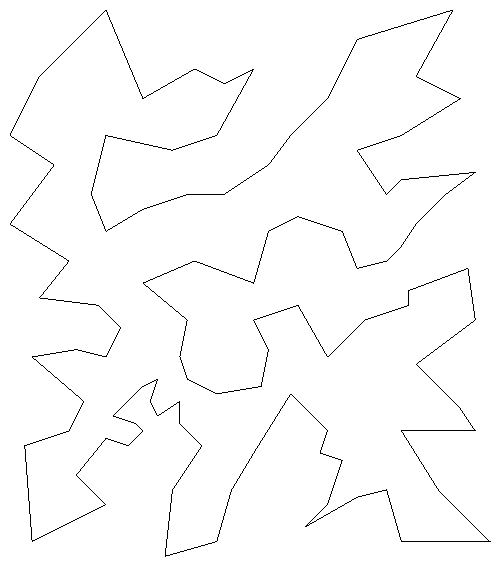
\includegraphics[width=0.5\textwidth]{sim_ex.pdf}}
  \subfloat{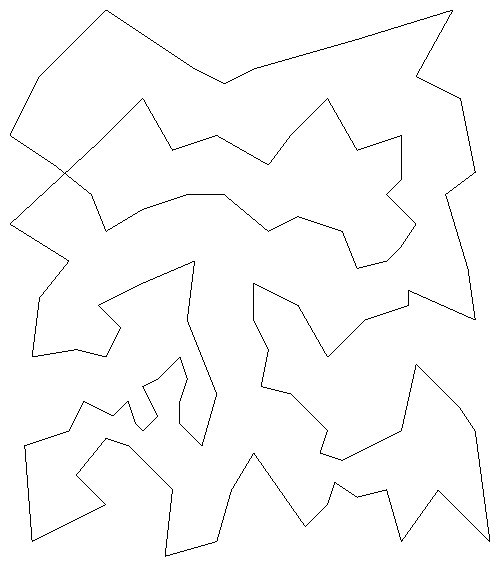
\includegraphics[width=0.5\textwidth]{gen_ex.pdf}}
  \caption{Optimised routes using simulated annealing (left) and a genetic algorithm (right). This is an example from eil101, an optimisation problem with 101 cities which will later be discussed in more detail. }
  \label{fig:example}
\end{figure}

\section{Methods}
In this report we use two different methods: simulated annealing and genetic algorithms. Both methods are widely used for finding optimal structures and configurations of systems, such as crystal structures, hard sphere problems, polymer and genome optimisation and the TSP. We will first describe the principles of both methods and then focus on the specific implementation for the TSP.

\subsection{Simulated Annealing}
Simulated annealing is an algorithm developed from a physics world view. The problem is finding the global minimum energy, given a (usually enormous) energy landscape, where each point in the landscape corresponds to a certain energy. The term simulated annealing comes from the heating of crystal structures and subsequently cooling down these structures slowly. If the temperature of such a system decreases slowly enough, the crystal structure will condense in a state which, in terms of energy configuration, is nearly (or fully) optimal. This process is called annealing and since this process can be mimicked for other problems which have to be solved by the computer, it is called simulated annealing.\\
In simulated annealing the temperature of the system is decreased gradually, so the simulation consists of many plateaus, all of which have a fixed temperature. Within each of these plateaus one would like to search the energy landscape for minima. This searching is done in a specific way, namely with the so called Markov chain Monte Carlo methods. A Markov Chain is simply a process in which the system goes through a chain of subsequent states (a state of the system corresponds to a point in the energy landscape), where the number of states is finite and the system is memory-less, so the current state does not depend on the previous states. The transition from one state $i$ to another state $j$ is characterised by transition probabilities $P_{ij}$. The Markov Chains that are used in this report are homogeneous (time-independent), irreducible, aperiodic and satisfy detailed balance. Irreducibility guarantees that the whole energy landscape can be explored, aperiodicity makes sure any state can appear at any point in the chain and detailed balance makes sure there is a steady state distribution for every point in the chain. In the case of simulated annealing the steady state distribution is a function of the temperature. \\
We can divide the transition probability for the Markov chain in two parts, a probability $G_{ij}$ to generate a new state $j$ from $i$ and a probability $\Gamma_{ij}$ to accept this new state. If we take $G_{ij} = G_{ji}$ and let all the states have an equal probability to be generated, $\Gamma_{ij}$ can be solved using information about detailed balance, see \cite{book}, as:
\begin{equation}
  \Gamma_{ij} = \text{min} \{ \frac{p(j)}{p(i)},1 \}
\end{equation}
where $p(x)$ is the desired distribution for the states. This is called the Metropolis algorithm (it can also be defined with $G_{ij}$ arbitrary). In the case of simulated annealing usually the Boltzmann distribution is chosen as the desired distribution, since it is a function of temperature. The acceptance probability for a new proposed state then becomes:
\begin{equation}
  \Gamma_{ij} = \text{min} \{ e^{-\Delta E/T},1 \}
\end{equation}
where $T$ is the reduced temperature of the system and $\Delta E$ the energy difference between state $i$ and state $j$.\\

The above algorithm can also be applied for the TSP. A state corresponds to a possible route, its energy corresponds to the length of the route. We then proceed as follows:
\begin{enumerate}
\item 
  Start at a temperature $T_{\text{max}}$ and generate a random route.
\item
  Generate a new tour from the previous one by applying Lin 2-opt transition (for an explanation see below).
\item
  Accept the new tour with probability $\Gamma_{ij}$, this requires computing the length of both the old and the new tour.
\item
  Repeat steps 2 and 3 a number of times $N_{\text{steps}}$, the number of steps in one Markov chain.
\item
  Lower the temperature in a suitable way (for an explanation see below) and repeat steps 2,3 and 4 until the energy does not change anymore for a number of Markov chains.
\end{enumerate}

A proposed route is generated from the current route by applying Lin 2-opt transition. In this method one selects two cities randomly in the current route. Then the cities which are visited in between this two chosen cities are visited in reversed order. This then becomes the new route. By chosen the two cities randomly, reaching all of the state space is guaranteed. Next this has to be repeated a number of times, which constitutes one Markov chain. Because for each temperature the Markov chain has to equilibriate the length of the Markov chain is usually a function of temperature, the higher the temperature, the longer it takes for the Markov chain to equilibriate. The TSP is a special problem in the sense that it searches for the minimum route and not the average length of the route, so in this case we can keep lowering the temperature until state changes are highly unlikely and the system is trapped in a certain state. This state will then be the state with the minimum energy, hence route length.\\
The above will only work when the temperature is lowered slowly enough. If the temperature is lowered fast, the system will get stuck in a local minimum, instead of a global one. This can still happen with slow temperature decrease but hopefully the local minimum in which the system gets stuck will then be very close to the global minimum. There are different ways of choosing a cooling schedule for the system, one of the most commonly used is a fractional one, where $T_{n+1} = \alpha T_{n}$ with $ 0 < \alpha < 1$ \cite{book}. There are other ways of cooling the system but the difference is not that important as long as the cooling goes slow enough. The cooling schedule should start at a certain temperature $T_{\text{max}}$ and end when the minimal route does not change anymore for a number of Markov chains. Since the temperature should be on the order of $\Delta E$ in order to get nonzero transition probabilities, generating a number of random routes before the actual simulation and calculating the maximum energy differences is a good measure. Once the maximum energy $\Delta E_{\text{max}}$ is calculated we can use $T_{\text{max}}$ = 10 $\Delta E_{\text{max}}$. The factor 10 is for making sure we are not excluding routes which have a very large energy differences but were not generated to determine $T_{\text{max}}$.

\subsection{Genetic algorithms}
Genetic algorithms is a broad field consisting of numerous algorithms all based upon mimicking the process of natural evolution. The algorithms are based upon the principles similar in the concept 'Survival of the fittest'. A simulation consists of generating subsequent generations, where a generation consists of a subset of states of the system. The 'best' states will become parents and produce offspring, the offspring constitutes the subset of states which are present in the next generation. By carefully selecting and applying mutations and crossovers (like in DNA replication) subsequent generations can become more and more healthy, meaning they converge towards a global maximum or minimum, that is often desired. A genetic algorithm usually consists of the following steps \cite{wiki}:
\begin{enumerate}
\item 
  \textbf{Initialisation}: At the start of the simulation a population is chosen from all possible states.
\item
  \textbf{Selection}: In each generation, a subset is chosen to produce offspring, called the parents. Often the parents are chosen based upon their fitness, which is a value depicting how healthy they are. There are numerous ways to select parents, we will give the methods applicable to the TSP and used in this report below.
\item
  \textbf{Crossover}: The parents procreate and produce offspring. There are again numerous ways to combine information of the parents and produce offspring. We will not cover all these possibilities here but consider the methods used in this report below.
\item
  \textbf{Mutation}: The offspring does not exactly copy the relevant information from the parents, but also has some parts changed randomly, again we will make this more specific below.
\item  
  \textbf{Repeating}: Steps 2, 3 and 4 are repeated for a number of generations.
\end{enumerate}

The above algorithm is a general description of a genetic algorithm. A specific implementation for the TSP is used in this report. We start with a population of 10000 random units, where each unit is a possible route between cities. For each unit we calculate a fitness function, which is, similar to the case of simulated annealing, the length of the route. Note that in this case a low value for the fitness means a better unit, assuming our desired route is the smallest possible one. Next is the selection step, where parents have to be chosen from the population. The following method is implemented in this report:
\begin{enumerate}
\item
  Randomly pick two parents from some percentage of the population with the lowest fitness function. In this way only the best units from the population get selected for producing offspring.
\end{enumerate}
The next step is producing offspring by combining the parents and applying crossover operators. Commonly used operations are single and multiple point crossovers, where a random site is selected on both parents, and the part left of this site of the first parent is glued to the part right of this site of the second parent. This will produce offspring of the right dimensions but the problem in the case of the the TSP is that the offspring may contain cities which are visited either zero times or more than one time, making this operation not suitable. Instead we use a method called a Greedy algorithm \cite{Greedy}, which works as follows:
\begin{enumerate}
\item 
  Pick a random city, this is the starting city of the route for the offspring. Call this random city the current city.
\item
  Look at the adjacent cities of the current city in both parents, this gives a maximum of four neighbours. Look at which of these four neighbours is closest to the current city and make this the next visited city in the tour of the offspring. If this city is already visited in the offspring tour, take the next closest one, and repeat until you have considered all neighbours. If all the neigh boring cities are already visited in the offspring tour, pick a random city and make that the next visited city.
\item
  Make the next visited city of the last step the current city, repeat step 2.
\end{enumerate}
This algorithm makes sure no city is visited twice in constructing a tour for the offspring. There is a major downside for this method, namely that this method is purely based upon local optimisation. And it is often useful to also explore methods which may not be very optimal on a local level, but might turn out to be very well suitable on a global level. A way to take care of this is by using mutation. After the creation of offspring from two parents the visited cities in the tour are randomly switched, with a fixed probability equal to $\frac{1}{N}$, where $N$ is the number of cities. This will give on average one mutation in every offspring. We will also set the mutation rate to zero and see what happens in that case.\\
Another extra feature not yet discussed (because it is often left out) is elitism. This usually occurs in the crossover step where the best parents are selected and converted to offspring without any crossover operations. In this report we use elitism with the best individual only from the population. This guarantees that the most optimal route found will decrease as the number of generations increases, because the best sample of every generation will be carried over.\\
Determining when to stop the simulation can be tricky with this algorithm, since when the mutation rate is not equal to zero, the system can always jump in a lower minimum after some number of generations. A rule of thumb that is used in this report is that when the fittest individual (so the most optimal route) does not change for 1000 subsequent generations, the simulation is stuck and will terminate, with the final result being that fittest individual.

As mentioned in the theory section, there is a library available with TSPs with solutions. This we can use to test the convergence of our algorithms. In this case the analysis is simple, implement the cities and intercity distance and use both simulated annealing and genetic algorithms to find the minimal route and compare this with the minimal route given by the data. One could rerun both algorithms multiple times to check if the minimal route that is found by the algorithms stays more or less the same.\\
In the case when the minimal route is unknown, the analysis is less straightforward. A possible way would be to run both algorithms until the stop criterion, which is when a number of subsequent Markov chains or generations give the same result for the fittest member. Especially in the case of a large number of cities ($N > 50$) the algorithms will get stuck on multiple local minima. One could then calculate the average of these minima and the standard deviation of all the minima to give a very careful estimate for the lower bound, for instance by postulating that probably the minimum will not be further away then twice the sample standard deviation from the absolute minimum found. This makes sense because the difference between the minima found by the algorithms will be routes that are very close together in terms of total distance (but may look very different) and it is highly unlikely there is one route which is much shorter than all those routes. The best route found by the algorithms would still be the minimum of all the minima.

\section{Results}
The results section is roughly divided up in two parts. In the first part we consider randomly generated routes and try to get as close as possible to the minimal route. The second part uses data from TSPLIB to from which the optimal route is known. First we show and example of how the minimal route evolves over time for both algorithms, the result is shown in figure \ref{fig:data}.

\begin{figure}[H]
  \subfloat{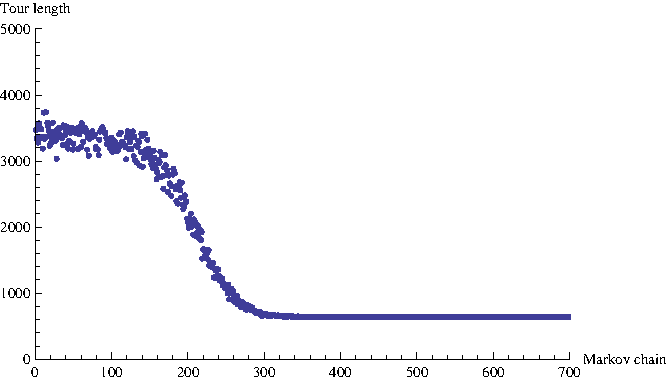
\includegraphics[width=0.5\textwidth]{sim_data.pdf}}
  \subfloat{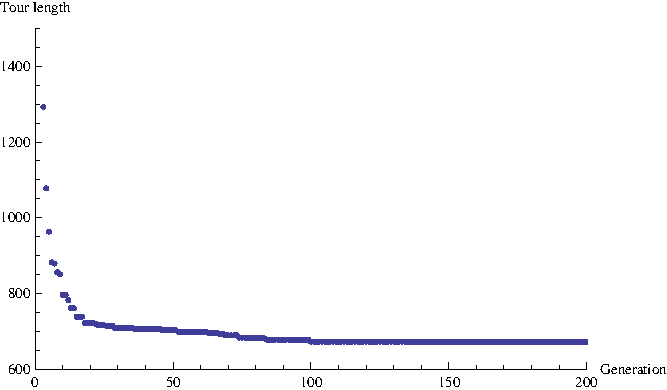
\includegraphics[width=0.5\textwidth]{gen_data.pdf}}
  \caption{The minimal route as a function of the Markov chain for simulated annealing and the minimal route as a function of generation for the genetic algorithm. Notice the faster but worse convergence for the genetic algorithm compared with simulated annealing. }
  \label{fig:data}
\end{figure}

\subsection{Randomly generated routes}
In this section we consider randomly generated routes. First the cities are initiated randomly on a square with area 1. The a distance matrix is generated based on the city locations. We apply both simulated annealing and genetic algorithms as described in the 'Methods'  section, with the following parameters and cases:
\newline
Simulated Annealing:
\begin{itemize}
\item 
  Number of random routes to set initial temperature: $10^6$.
\item
  Temperature decrement: $\alpha = 0.975$, this corresponds to a 2.5\% temperature decrease every Markov chain.
\item
  Length of Markov chains: 10000, 50000 or 100000, this number is not temperature dependent because for small enough decrements of the temperature (which is the case here) thermalisation of the Markov chain is very quickly achieved if thermalisation is already achieved for the previous Markov chain, since the temperature can then be regarded as being continuous, and so the corresponding Boltzmann distribution changes also continuously. Since we are only interested in the eventual outcome and the the initial temperature is set very high, it does not make much difference if the first few Markov chains are not fully thermalised.
\item
  Number of Markov chains with the same minimal route before stopping the simulation: 250. Every Markov Chain the optimal route is computed for that chain using the second half of the Markov chain only (to avoid measuring in non-equilibrium). If the optimal route (and hence the length of the route) stays the same for 250 consecutive Markov Chains, the simulation is terminated.
\end{itemize}
Genetic Algorithm:
\begin{itemize}
\item 
  Population size: 10000
\item
  Percentage of fittest individuals that are considered for producing offspring: 25\%, 10\% or 1\%, so given a population size, these are the percentages of the individuals that can be picked randomly to produce offspring.
\item
  Number of elitists: 1, to ensure the optimal route is monotonic descending as a function of generations.
\item
  Number of generations which same optimal route before halting simulation: 1000
\item
  Probability of mutation: 1/N or 0
\end{itemize}

So we choose here to vary the length of the Markov chain for simulated annealing, and the selection percentage and the mutation probability for genetic algorithms. Other quantities are kept fixed throughout all following results for simplicity. We run the simulation for 10, 100 and 250 randomly initialised cities on the unit square, keeping the seed for the city positions the same to ensure a fair comparison. We measure the length of the minimal route for both algorithms and repeat the experiment 25 times to find the mean and the sample standard deviation as well as the minimum of all the minima. This is used to give an estimate for the lower bound, given by the minimum of the minima minus twice the sample standard deviation. The results for this simulation are given in the tables below:

\begin{table}[H]\footnotesize
  \centering
  \begin{tabular}{l | *{4}{c} r}
    \hline
    \multicolumn{6}{c}{Simulated annealing} \\
    \hline
    N & avg. min & sample std & avg. steps & min & lower bound \\
    \hline
    \multicolumn{6}{c}{$N_{\text{chains}}$ = 10000} \\
    \hline
    10 & 2.58476 & 0 & 6.96 & 2.58476 & 2.58476\\
    100 & 7.96223 & 0.069875 & 249.64 & 7.87466 & 7.73491\\
    250 & 12.1977 & 0.172062 & 339.48 & 11.8961 & 11.5520\\
    \hline
    \multicolumn{6}{c}{$N_{\text{chains}}$ = 50000} \\
    \hline
    10 & 2.58476 & 0 & 3.2 & 2.58476 & 2.58476\\
    100 & 7.92243 & 0.0369846 & 237.76 & 7.87466 & 7.80069\\
    250 & 11.8919 & 0.0785142 & 312.92 & 11.7398 & 11.5828\\
    \hline
    \multicolumn{6}{c}{$N_{\text{chains}}$ = 100000} \\
    \hline
    10 & 2.58476 & 0 & 2.44 & 2.58476 & 2.58476\\
    100 & 7.90541 & 0.0190712 & 230.04 & 7.87466 & 7.8365\\
    250 & 11.8704 & 0.0963631 & 314.96 & 11.7362 & 11.5435\\
    \hline    
  \end{tabular}
  \caption{Simulated annealing: the average minimum, the sample standard deviation, the average number of steps after which these minimum was achieved, the minimum of the minima and the lower bound for the minimum.}
  \label{tab:sim_random}
\end{table}

\begin{table}[H]\footnotesize
  \centering
  \begin{tabular}{l | c c c c c | c c c c r }
    \hline
    \multicolumn{11}{c}{Genetic algorithm} \\
    \hline
    N & avg. min & std & avg. steps & min & lower bound & avg. min & std & avg. steps & min & lower bound\\
    \hline
    \multicolumn{1}{c}{} & \multicolumn{5}{c|}{selection = 25\%, mutation off} & \multicolumn{5}{|c}{selection = 25\%, mutation on} \\
    \hline
    10 & 2.58476 & 0 & 2.84 & 2.58476 & 2.58476 & 2.58476 & 0 & 3.24 & 2.58476 & 2.58476\\
    100 & 8.25875 & 0.0948193 & 378.8 & 8.06633 & 7.87669 & 8.22935 & 0.0873101 & 335.24 & 8.13263 & 7.95800\\
    250 & 12.1491 & 0.0808337 & 120.88 & 12.0092 & 11.8475 & 12.1858 & 0.0725029 & 51.92 & 12.0496 & 11.9046\\
\hline
    \multicolumn{1}{c}{} & \multicolumn{5}{c|}{selection = 10\%, mutation off} & \multicolumn{5}{|c}{selection = 10\%, mutation on} \\
    \hline
    10 & 2.58476 & 0 & 2.36 & 2.58476 & 2.58476 & 2.58476 & 0 & 2.48 & 2.58476 & 2.58476\\
    100 & 8.20183 & 0.0269283 & 68.4 & 8.15967 & 8.10581 & 8.17947 & 0.0518344 & 118.48 & 8.12043 & 8.01676\\
    250 & 12.1347 & 0.0713821 & 111.24 & 11.9973 & 11.8545 & 12.1254 & 0.0765085 & 229.96 & 12.0429 & 11.8899\\
    \hline
    \multicolumn{1}{c}{} & \multicolumn{5}{c|}{selection = 1\%, mutation off} & \multicolumn{5}{|c}{selection = 1\%, mutation on} \\
    \hline
    10 & 2.58476 & 0 & 2.32 & 2.58476 & 2.58476 & 2.58476 & 0 & 2.48 & 2.58476 & 2.58476\\
    100 & 8.26692 & 0.119716 & 16.16 & 8.01992 & 7.78049 & 8.11368 & 0.0789699 & 135.08 & 7.95471 & 7.79677\\
    250 & 14.8162 & 0.871053 & 27.68 & 13.6244 & 11.8823 & 12.7541 & 0.28391 & 120.72 & 12.2737 & 11.7059\\
    \hline    
  \end{tabular}
  \caption{Genetic algorithm: the average minimum, the sample standard deviation, the average number of steps after which these minimum was achieved, the minimum of the minima and the lower bound for the minimum}
  \label{tab:gen_random}
\end{table}

The table for simulated annealing shows a clear pattern, the larger the Markov chains, the more accurate the solution becomes. The minimum of the solutions for $N$ = 10 and $N$ = 100 are the exact solutions for simulated annealing, so in those cases the lower bound does not make much sense. The average number of steps is slightly decreasing for increasing Markov chain length, which makes sense. But from the table it is clear that large Markov chains lead primarily to better solutions and not so much to faster convergence.\\
In the table for genetic algorithms we see first of all that the solution is exact for $N$ = 10, and this holds for all scenarios which were tested. For a higher number of cities the result is more interesting. For $N$ = 100 the results perform better for a selection of 1\% than for a selection of 10\%, while it is the other way around for $N$ = 250. A possible explanation for this is that the crossover algorithm used is very local and with a selection of 1\% the population tends to go to a very small subset close (but not at) the global minimum. For the case of $N$ = 250 this selection of 1\% goes much too fast and closes off interesting parts of the search space, while for lower city sizes the state space is much smaller and hence this quick convergence to a small subset might lead actually to the right part of the state space (i.e. close to the global minimum). This suggests it might be wise to implement a selection criterion dependent on the number of cities, more on this in the discussion below.\\
Another interesting thing is that the mutation might not be that influential in the way this model is set up. The populations converge without mutation to a value just slightly above the value with mutation, with the added feature that the simulations are much shorter for high city numbers, since the number of steps drastically decreases. This is again unexpected behaviour, the reason might be that almost all the mutations get rejected and will not make it into the selection pool in the next generation, this is also supported by the fact that for a selection of 25\% the number of steps is less when mutation is implemented, contrary to the other two cases.

If we compare both algorithms it is clear that simulated annealing gives much better results. The average of the results lies closer to the global minimum and there is a clear pattern in the case of simulated annealing while in the case of genetic algorithms much more factors play a role. Though the tables do not tell this, the simulated annealing is also much, much faster in terms of execution time, namely around a factor of five. Though it is hard to compare the two methods since the parameters are not easily linked to each other (e.g. there is not a clear one-to-one correspondence between Markov chain - generation and temperature - selection process) the fact that simulated annealing produces much better results in much less time we can conclude that with this specific setup the simulated annealing works much better and is a preferable method over the genetic algorithm. 

\subsection{Data from TSPLIB}
Next to randomly generated cities we can also get coordinate maps and distance table from TSPLIB, available from \cite{TSPLIB}. The following data sets are chosen:
\begin{itemize}
\item 
  Dantzig42: a 42 city problem, each city represents the capital of a continental state of the US. Data consists of an intercity distance matrix.
\item
  Berlin52: a problem of visiting 52 sights in Berlin. Data consists of sight coordinates.
\item
  eil101: a 101 city problem. Data consists of city coordinates.
\item
  pr439: a 439 city problem. Data consists of city coordinates.
\end{itemize}

Like in the previous example, we again run the simulation both with simulated annealing and genetic algorithms, but this time we will not do statistics because the lower bound for these cities is already known. We compute the minima 25 times and take the minimum of these minima as the best estimate. For simulated annealing we used the case with a Markov chain of length 100000. For genetic algorithms we used mutation and a selection of 10\%, based on the results in the previous section. The table below shows the results:

\begin{table}[H]
  \centering
  \begin{tabular}{ l | *{4}{c} r}
    \multicolumn{2}{l}{} & \multicolumn{2}{c}{Simulated annealing} & \multicolumn{2}{c}{Genetic algorithm} \\
   \hline
   & Optimal tour & Shortest tour & Deviation & Shortest tour & Deviation \\
   \hline
    Dantzig42 & 699 & 699 & 0 (0\%) & 699 & 0 (0\%) \\
    Berlin52 & 7542 & 7544.37* & 2.37 (0.03\%) & 7544.37* & 2.37 (0.03\%) \\
    eil101 & 629 & 640.212* & 11.212 (1.8\%) & 647.176 & 18.176 (2.9\%) \\
    pr439 & 107217 & 108120 & 903 (0.8\%) & 110854 & 3637 (3.4\%)\\
    \hline    
  \end{tabular}
  \caption{Results for different city problems, the known shortest path length, the minimum over 25 simulations and the relative difference (in per cent).\\
* These values are the global minima, for an explanation see the text below.}
  \label{tab:sim_map}
\end{table}

From this table we see again, like in the previous section, that the simulated annealing outperforms the genetic algorithm. However, some remarks must be made. For some reason, if the input is in the form of a coordinate list of cities (this is the case for all problems except Dantzig42), the computed minimum does not coincide with the minima given by the authors of TSPLIB. The statement that the minima with a * that were computed are the global minima is based upon the following three arguments:
\begin{itemize}
\item 
  Even though the total length of the route is not the same, the route that is found in the case of a * value coincides exactly with the route found by the authors of TSPLIB.
\item
  An evaluation of the route in Mathematica using the function FindShortestTour gives no results better than the * result for all possible methods implemented in Mathematica.
\item
  Fellow students working on the same problems have also found the same route as the authors of TSPLIB, but the length of those routes was also equal to the * value that is reported here.
\end{itemize}
For pr439 the authors of TSPLIB do not give an optimal route, only the length of the optimal route, so it is not clear whether the minimal route found with simulated annealing (108120) is the global minimum, though it is likely not since the spreading in simulations in that case is fairly big (not shown in the table).

\section{Conclusion and Discussion}

We tested two algorithms to solve the TSP. We used genetic algorithms with Greedy crossover, elitism, mutation and random selection from the best portion of parents. We also used simulated annealing with different Markov chains and a fixed temperature profile. From table \ref{tab:gen_random} and table \ref{tab:sim_random} we can conclude that the genetic algorithm has a much poorer performance when implemented as in the section Methods, as the simulated annealing algorithm. This is again confirmed by table \ref{tab:sim_map}. We find some problem dependent behaviour for the genetic algorithm, since very strict selection seems to be preferred for small problems, while non-strict selection seems to be preferred for larger problems, which can be explained by the larger state space for larger problems and the strong local focus of the Greedy algorithm. The application of the two algorithms using known problems from TSPLIB did not give much more insight, since the global minima found do not coincide with the global minima reported by the authors. However, there are strong reasons to believe that the results reported in this report are correct.

In this particular setup it is clear that simulated annealing is the preferred method, however there exist a lot of different implementations of genetic algorithms. This Greedy algorithm is certainly not the best way. In \cite{Greedy} the authors proposed an improved Greedy algorithm which I was unfortunately not able to implement due to time restrictions. Their main point is to tackle the problem of the focus on local convergence in the Greedy algorithm. Another way to make the genetic algorithm perform better is by making it adaptive. One could for instance change the selection process if the population tends to get to uniform, which is often the case, especially when selecting only 10\% of 1\% of the population. Due to the nature of the Greedy algorithm, two parents with the same route always produce a clone of themselves as offspring and hence when most of the parents are either almost or fully the same, the system will get stuck. Mutation should unstuck the system, but in practicality the form of mutation implemented in this report (on average one per offspring) is not very strong, especially not with the chosen selection procedures. The probability that a mutation will survive in the next generation is very small because usually mutations do not have a standalone benefit and so will not be chosen in the next generation as a parent (just as in nature mutations have to occur simultaneously or across different parents to produce more valuable offspring). So there is a lot of room for improvement on the side of genetic algorithms.

Considering simulated annealing the way it was set up worked reasonably well. One of the parts that might need an improvement is the Lin 2-opt transition. This transition is not temperature dependent, so that means that if the system has advanced far enough, most routes that will be generated by this transition are not going to be accepted. It might be a good idea to decrease the allowed distance between two randomly chosen cities in between which the Lin 2-opt transition is performed as a function of temperature. This will cause the transitions to be much smaller in terms of cities swapped for low temperatures, and in general these small transitions will lead to a new route with a fairly low (or lower) cost with respect to the current route and thus a higher acceptance probability. However since the termination of the simulation is dynamic as well and does not have a fixed lower temperature bound, I found this difficult to implement in a clever way. Earlier versions of the algorithm I wrote had both a start temperature and a lower bound for the temperature, in this case the distance between cities to perform a transition might have been a linear function with temperature for instance. I computed this lower  bound for the temperature in the same way as I did for the upper bound described in the 'Methods' section, but I found that sometimes the simulation would terminate when the system was still working towards an equilibrium, so I discarded the method for the 'safer' method of terminating the simulation when no improvement has been made in 250 Markov chains.

The implementation of both simulated annealing and genetic algorithms involves setting a list of parameters. While some of the parameters are varied explicitly in this report, some others were tested as well. Usually though they were tested on a small toy problem, usually a 10 random city TSP. I found it difficult to tweak the parameters correctly, and to justify the chosen values, since most parameters have optimal values which are highly dependent on the problem. I have read some reports on this, and for instance the placement of cities (keeping the number of cities constant) can already influence greatly how the parameters should be set, it can even force you to change algorithms in the case of genetic algorithms. Below is a list with the most important parameters used for the genetic algorithm and a short explanation (or sometimes just 'rule of thumb') why they are used:

\begin{itemize}
\item 
  Population size: 10000, this number is based upon literature values, but I have to admit it is quite arbitrary. The size is also coupled to the selection criteria that are used.
\item
  Percentage selected for offspring: 1\%, 10\% or 25\%, originally in the first versions this was fixed at 25\%, but I noticed a significant improvement with lowering it, especially for low city numbers. Setting a percentage higher than 25\% slowed the simulation down and produced worse results (for $N$ = 100).
\item
  Number of elitist: since chosen the elitist number is a study on its own, I decided to keep it simple and just take 1 elitist per generation. This ensures that the best solution so far stays in the system, which was my primary reason for introducing elitism.
\item
  Number of generations with same optimum before terminating simulation: 1000, this is purely done by trial-and-error. Sometimes after 1000s of generations the system will suddenly change because a suitable mutation comes along, but since my system is not adaptive this takes usually a lot of time. A value of 1000 makes sure that the simulation does not stop too quickly, but at the same time it does not take up too much time, which was also a consideration for me.
\item
  Probability of mutation: 0 or 1/$N$, this is again a literature standard. I did set the value to 2/$N$ and 5/$N$ to test what would happen and it makes the system unstable (losing good solutions) and it takes much more time to converge, maybe coupled with a strict selection this would be a good setting though.
\item
  Number of simulations: 25, this is purely time-based.
\end{itemize}

Before working on the TSP I wanted to do the 'charges on a sphere' problem using genetic algorithms. The idea is from the paper \cite{gen1} in which they use a population of size 16, consisting of 16 configurations of charges on a sphere. Every generation they select the four best parents, randomly cut them in half and combine them to form 16 offspring spheres. These spheres are then locally optimised by conjugate gradient methods and the best 4 are again selected to be the parents in the next generation. The authors showed that this method works extremely fast and well, where only a few generations were enough to produce results close to the global minima. I started implementing this method but it turned it was far too much work to be able to do in two weeks, especially the cutting and gluing of the spheres is a complicated procedure, since there is a constraint that the total number of particles has to be constant. Nevertheless, the paper is very interesting and I have added it to the zip file.

\begin{thebibliography}{15}
\bibitem{book}
  Ross, S.M., \emph{Simulation}, 2006, Academic Press
\bibitem{TSPLIB}
  http://comopt.ifi.uni-heidelberg.de/software/TSPLIB95/
\bibitem{wiki}
  http://en.wikipedia.org/wiki/Genetic\_algorithm
\bibitem{Greedy}
  Wang, Z., Duan,H. Zhang, X., \emph{An Improved Greedy Genetic Algorithm for Solving Travelling Salesman Problem}, ICNC '09, 374-378
\bibitem{gen1}
Morris, J.R., Deaven, D.M., Ho, K.M., Physical Review B, 1996, Vol. 53, Number 4, 1740-1743 
\end{thebibliography}

\end{document}
